\chapter{Introduzione alla complessità}
Tutti i sistemi fisiologici sono caratterizzati dalla loro specifica \textbf{complessità}, ogni modello rappresenta un'\textbf{approssimazione} della complessa realtà. Il modello sviluppato deve tenere conto di: 
\begin{itemize}
    \item La complessità intrinseca che è stata semplificata
    \item Disponibilità dei \textbf{dati} necessari per stimare i parametri
\end{itemize}
Quando si guarda un sistema bisogna comprendere la complessità di quest'ultimo e semplificarla attraverso i dati a disposizione.
Quando si ha un sistema complesso ci si concentra su un "situation focus", dal sistema bisogna estrarre le relazioni rilevanti. Queste ultime possono essere utilizzate per spiegare (in modo approssimativo) il sistema, tuttavia non lo descrive completamente: tutti i modelli sono sbagliati ma alcuni sono utili. Conoscere i limiti del modello è essenziale per migliorarlo.

\section{Complessità dell'organismo umano}

%aggiungi foto slides 

L'organismo umano è un sistema multi-input, multi-output controreazionato. Nel modello vengono presi in considerazione disturbi (fisici o mentali) e constraints ??. Nonostante la complessità del modello è comunque semplificato rispetto al sistema reale. La complessità dipende da vari fattori:
\begin{itemize}
    \item Il numero di elementi del sistema 
    \item Interconnessione tra gli elementi
    \item Il comportamento del sistema \textbf{stocastico} e non deterministico
    \item \textbf{Asimmetria} delle relazioni del sistema (per esempio la crescita differenziale delle cellule)
    \item Vincoli non olonomici (le varie parti del sistema assumono indipendenza) 
    \item Processi tempo-varianti
\end{itemize}

I concetti chiave legati alla complessità fisiologica sono feedback.

\subsection{Feedback}
Il feedback è una proprietà fondamentale dei sistemi biologici che permette il controllo e la regolazione, è quindi un ingrediente fondamentale della complessità che caratterizza i sistemi fisiologici. Il feedback è sinonimo di mutua causalità: la variabile X ha un effetto sulla variabile Y e viceversa Y ha un effetto su X. 
\subsubsection{Negative feedback}
Nel feedback negativo un incremento nella variabile X porta ad un incremento della variabile Y e tale incremento nella variabile Y porta un decremento nella variabile X. Questo permette di mantenere variabili nel range basale, come per esempio il metabolismo del glucosio. Dal processo di digestione dei carboidrati produciamo glucosio che viene immesso nella circolazione (aumento di X), il pancreas produce in risposta insulina (aumento di Y) antagonista del glucosio che porta all'assorbimento del glucosio da parte delle cellule (feedback negativo a X). Il meccanismo di feedback negativo crea \textbf{stabilità}.

%immagine ciclo glucosio

\subsubsection{Positive feedback}
Nel feedback positivo un incremento nella variabile X porta ad un incremento della variabile Y e tale incremento nella variabile Y porta ad un ulteriore incremento nella variabile X. Questo meccanismo non è diffuso nei sistemi biologici poichè causa \textbf{instabilità}. Uno dei pochi esempi di feedback positivo sono le contrazioni uterine del parto. La spinta della testa del bambino sulla cervice genera ad una stimolazione neurologica che porta alla secrezione di ossitocina, quest'ultima entra nel flusso sanguigno e porta alla stimolazione delle contrazioni uterine. 

\subsubsection{Feedback intrinseco}
Nelle reazioni chimiche, si parla di feedback intrinseco se il tasso di decremento della concentrazione di A è proporzionale solo alla sua concentrazione; non intervengono quindi fattori esterni. 
\begin{equation}
    \frac{dC_A}{dt}=-kC_A
\end{equation}
Dove $C_A$ è la concentrazione chimica di A e k è la costante di flusso della reazione. 

%foto feedback intrinseco 
\subsubsection{Feedback nei sistemi dinamici}
Quando il sistema di feedback viene a mancare si ha il passaggio dalla condizione di salute alla patologia. Per esempio il diabete è causato dal malfunzionamento del sistema di feedback dell'insulina. Nel diabete di tipo 1 il ramo di andata, non viene prodotta insulina. Nel diabete di tipo 2 non funziona la parte di controreazione, viene prodotta insulina ma non avviene l'assorbimento al livello cellulare. 
%foto insulina

\subsubsection{Altri tipi di feedback}
L'omeostasi è un processo che dipende dal tempo, questo significa che non possiamo avere solo un feedback di tipo proporzionale ma anche di tipo derivativo e integrale. Per esempio se avessi delle variazioni molto veloci (spike) non verrebbe prodotta abbastanza insulina.
Il feedback di tipo \textbf{proporzionale} può dar luogo a ritardi nell'ottenimento dell'effetto della controreazione.
Il feedback di tipo \textbf{derivativo} permette di tenere conto delle variazioni temporali, e della velocità di variazione, dei valori.
In alcuni sistemi compare anche il feedback di tipo \textbf{integrale} che permette di aggiustare il valore a regime della variabile una voltache è stato applicato il feedback. Si applica un feedback proporzionale all'integrale della differenza tra il valore della variabile controllata e il suo valore atteso. 
%diagramma di feedback

\subsection{Controllo}
I pattern di regolazione e controllo che avvengono nei sistemi
fisiologici sono molti e vari e caratterizzano la complessità
dell'organismo umano (interni all'organismo - \textbf{omeostasi}, o
esterni – \textbf{gestione stimoli} in ingresso agli organi di senso). Gli strumenti di controllo per il mantenimento dello stato vitale sono:
\begin{itemize}
    \item Equilibrio statico e dinamico
    \item Regolazione lineare e non lineare
\end{itemize}
Il nostro corpo attua il controllo attraverso due strumenti:
\subsubsection{Enzimi}
Gli enzimi sono catalizzatori biologici delle reazioni chimiche che avvengono nell'organismo umano (aumentano la velocità di reazione):
\begin{equation}
    E+S\longleftrightarrow X \longrightarrow E +P
\end{equation}
Questa è l'equazione di bilancio delle masse dove l'enzima E e il substrato S formano il complesso enzima-substrato XX che a sua volta decompone nell'enzima originale e nel prodotto della reazione P. Il modello del controllo tramite enzimi è complesso e deve essere applicato a tutte le reazioni. 
\begin{figure}[h!]
    \centering
    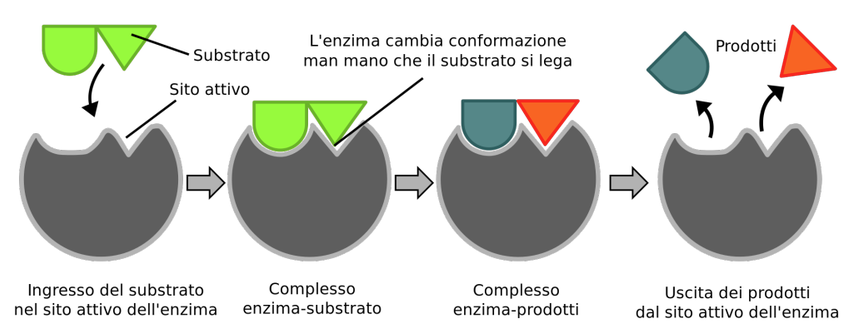
\includegraphics[width=0.75\linewidth]{immagini/enzima.png}
    \caption{Reazione catalizzata da un enzima}
    \label{fig:placeholder}
\end{figure}
\subsubsection{Ormoni}
L'altro processo di controllo avviene attraverso la produzione di ormoni secreti da ghiandole endocrine. Esistono vari tipi di azione ormonale che svolge il nostro corpo: 
\begin{itemize}
    \item \textbf{Azione cinetica}, agisce sulle concentrazioni
    \item \textbf{Azione metabolica}, agisce sui processi metabolici
    \item \textbf{Azione endocrino-cinetica}, 
\end{itemize}
\subsection{Gerarchia}
La struttura dell'organismo umano si
presta ad essere analizzato in termini
di gerarchia: dai geni, alle cellule,
agli organi, fino all'organismo. Ad ogni livello c'è un'azione di feedback e controllo, queste azioni sono coordinate a livello gerarchico e assicurano che gli organi siano in grado di sopportare disturbi normali e anomali sia in termini di grandezza che di scala
temporale.
 
Parte di questo processo è assicurato dalla \textbf{ridondanza}. Per mantenere la funzione in caso di danno ad uno dei due organi o per rendere più sofisticata la funzione. La ridondanza è presente anche nei sistemi di controllo degli organi

\medskip
Per quantificare i processi dinamici e interfacciarsi con la loro complessità è necessario effettuare delle misurazioni, i limiti su cosa può essere misurato sono:
\begin{itemize}
    \item Pratici, dipende dagli strumenti e dai punti di accesso
    \item Etici, dipende dal tipo di misurazione
\end{itemize}
Le misure non devono essere invasive, e per queste si utilizza un approccio diretto e metodi inferenziali.
